\documentclass[a4paper,12pt]{article}
\usepackage[utf8]{inputenc}

% Allow the change of line spacing
\usepackage{setspace}


\usepackage{graphicx}

%\usepackage{hyperref}
%\usepackage{breakurl}

%opening
%\title{Trainmining}
%\author{Grupo de Sistemas Inteligentes \\ Universidad Politécnica de Madrid}




\begin{document}
\newcommand\litem[1]{\item{\bfseries #1 }}
%\renewcommand{\abstractname}{Executive Summary}
%\begin{abstract}
%
%\end{abstract}

% Set line spacing to 1.5
\onehalfspacing

% Begin a new titlepage. Tit	lepages have special settings like the absence of page numbers.
\begin{titlepage}
\sffamily
% Set the text of the page to right-aligned until \end{flushright}
\begin{flushright}

% Set the space between right page border and text to 2.5cm
\rightskip=-1cm

% Show an image at this position

\includegraphics[scale=1]{./img/logoGSI.png} 
%\includegraphics[bb=0 0 204 110]{web40logo.png}

% Skip a little space
\bigskip
\bigskip
\bigskip



% Create a title for the document and write it in bold font
\LARGE{\textbf{Deliverable 1. Problem Scope.}}
% Again, do a line break
\linebreak
% Create a subtitle
\large{Description of the Project Context and Definition of Learning Goals.}

% Skip some space
%\bigskip
%\bigskip
%\bigskip
%\bigskip
\bigskip

% Write in very large letters
\LARGE{Grupo de Sistemas Inteligentes}
\linebreak
\large{Departamento de Ingeniería de Sistemas Telemáticos}
% Do a line break right after the \LARGE{...} text
\linebreak
% Write in large letters
\large{Universidad Politécnica de Madrid.}

% Skip some space
\bigskip
\bigskip
\bigskip
\bigskip
\bigskip
\bigskip

\large{Project Report}

% Skip some space
\bigskip

\normalsize{Madrid, September 2012}

% Skip some space
\bigskip
\bigskip
\bigskip
\bigskip
\bigskip
\bigskip
\bigskip
\bigskip
\bigskip
\bigskip
\bigskip
\bigskip
\bigskip
\bigskip
\bigskip
\bigskip

% Provide some author information
\normalsize{Authors:}
\linebreak
\large{Adrián Pérez Orozco}
\linebreak
\large{Álvaro Carrera Barroso}
\linebreak
\large{Carlos A. Iglesias Fernández}

% End right-alignment at this point
\end{flushright}
% End the title page
\end{titlepage}

%\maketitle

\pagenumbering{roman}
\section*{Executive Summary}
\addcontentsline{toc}{section}{Executive Summary} % si queremos que aparezca en el índice
This document describes the scope and potential outcomes of the project {\it Trainmining}. This project is developed by Thales Spain in collaboration with the research group {\em Grupo de Sistemas Inteligentes} (Intelligent Systems Group) of the
Universidad Politécnica de Madrid. The goal of the project is the application of machine
learning techniques for predicting alarms in the alarm system that have been developed by
Thales Spain. Machine learning techniques will be based on historical data coming from Thales Spain railway maintenance system which is on operation in several cities. 

The document provides a general overview of the railway maintenance system developed by Thales Spain, as well as the available historical data. In addition, the document describes potential learning goals for the application of machine learning techniques. Then, the document describes which are the learning goals Thales Spain is more interested in, and details potential machine learning techniques to achieve them. The selected learning goals are learning sequential alarm rules, and its usage is illustrated with a use case. 

\newpage
\tableofcontents % indice de contenidos
\addcontentsline{toc}{section}{Contents} % para que aparezca en el indice de 
\cleardoublepage
\addcontentsline{toc}{section}{List of Figures} % para que aparezca en el indice de contenidos
\listoffigures % indice de figuras

\cleardoublepage
\addcontentsline{toc}{section}{List of tables} % para que aparezca en el indice de contenidos
\listoftables % indice de tablas
\cleardoublepage

\setcounter{page}{1}
\pagenumbering{arabic}
%\chapter{Objectives and context definition}
\section{Introduction}\label{sec:context}
Maintenance is one of the most important tasks to assure the quality and correct operation of any kind of system. Even the highest quality systems, built by the best engineers to operate for long periods with the least possible human assistance, will eventually be exposed to damage or malfunction. In order to avoid the negative effects that system malfunction can produce, a significant amount of resources and effort is usually needed to be put on maintenance tasks. However, putting resources and effort on maintenance procedures might still not be enough if the procedures and strategies are not adequate and efficient.

Traditionally, we have discerned between two types of maintenance procedures:
\begin{itemize}
\item \emph{Corrective maintenance} is the most common approach, although it has very important limitations. With this approach, elements of our system are repaired or replaced once they have failed or worn out, to bring them back to operation. This usually means a high downtime in operation, as no actions are taken until our system is already malfunctioning.

\item \emph{Preventive maintenance} focuses on preventing these failures. Elements can be periodically examined and analysed in order to control their operation and perform simpler procedures to adjust them before reaching malfunction and downtime. This approach means much higher costs, as a significantly bigger amount of time is needed to monitor the elements on our system and correct them. However, as downtime means business losses in almost all cases, these higher costs usually pay back in terms of loss reduction.
\end{itemize}

A balance can be easily achieved by spending on preventive maintenance not more than the losses we would suffer from downtime if we were using a corrective approach.

However, the costs of preventive maintenance can be drastically reduced by optimising procedures and using the adequate techniques. For example, we can reduce the amount of variables and magnitudes we are monitoring (and which cost us money to monitor) if we know which ones give the better insight on the status on our systems. The same can be done with corrective maintenance. If we can somehow foresee which systems are going to fail, we can be prepared and reduce impact on our business even if we cannot do anything to prevent its failure.

In both cases, \emph{prediction} can be a key element for maintenance optimisation. Either we know which are the indicators of a system deterioration which we can repair, or we know which systems are going to fail and when to be prepared and optimise corrective procedures. We can even speak of a new type of maintenance - \emph{predictive maintenance} - which embraces several techniques to try and obtain this knowledge of future events.

\section{Project overview}
The project \emph{Trainmining} aims to design predictive maintenance techniques on already-existing maintenance stations of a railway network. These maintenance stations monitor different elements and subsystems over a railway line and raises alarms whenever a line element fails or requires human intervention. Additionally, maintenance workers perform different preventive maintenance procedures, gathering information about several parameters on each element and performing the appropriate actions when needed. Acquisition of values and determination of necessary actions is however not automatised within the maintenance stations, and workers have to manually perform these tasks.

In order to design \emph{predictive procedures} for the railway network, we have a big amount of event logs gathered by the maintenance stations, as well as registries filled by maintenance workers when performing preventive tasks. We will therefore try to extract, from that large amount of data, knowledge on how to predict future events from current observations

In this direction, \emph{Data Mining} techniques can be extremely useful in order to find relations between patterns in environment variables and the occurrence of events, or even relations between events themselves. These relations, which may at first not be apparent for the human mind, can be obtained through different automated learning processes, and thus infer markers which will act as indicators of when and how failures can happen. In order to extract this data we will need to count on a significantly high amount of event logs, gathered during previous years, on which we will apply said techniques.

\section{Project context}
For this project, Thales Group, a leader company in the development of railway systems in Spain is cooperating with the research group {\it Grupo de Sistemas Inteligentes} from the Universidad Politécnica de Madrid, with large expertise in the application of intelligent systems to real problems. Thales Spain has developed an advanced system called \emph{maintenance station}, which diagnoses, gathers and visualises different kind of events happening along the railway network. These maintenance stations comprise different advanced diagnosis systems, which can identify and report several kind of events happening along the lines which might require human intervention. These stations gather logs with all the events which have happened in the past, which will allow us to study and analyse the operation of these stations during the past.

At the moment of writing this document, we count on data of three maintenance stations: Antequera, Sevilla and Segovia, which are located in Spain. Each of these stations controls a different railway line, and have different diagnosis systems and characteristics, as shown in table~\ref{tab:stations}. In this table we see that the three lines we are working with are of different types and have different diagnosis systems. Specifically, Antequera and Segovia stations control high speed lines, while Sevilla station controls a commuter line. Different types of lines will have different elements and systems, and results are therefore expected to be different in both groups. Furthermore, supervised systems are different in all the three stations, which means that alarms received from each of them will not necessarily be the same. Details on number of events and time span of the available data is given on table~\ref{tab:data_details}.

\begin{table}
\begin{center}
\begin{tabular}{|c|c|c|}
\hline Name & Line type & Supervised systems \\ 
\hline Antequera & High Speed & SAM-E-L \\ 
\hline Segovia & High Speed & ERTMS (levels 1 and 2) \\ 
\hline Sevilla & Commuter & Diagnosis and Energy \\ 
\hline 
\end{tabular}
\\
-\\
ERMTS: European Rail Traffic Management System\\
SAM-E-L: Sistema de Ayuda al Mantenimiento para Ence (Local)\\

\end{center} 
\caption {Maintenance Stations} \label{tab:stations} 
\end{table}

\begin{table}
\begin{center}
\begin{tabular}{|c|c|c|c|c|}
\hline Maintenance Station & Number of events & Start date & End date & Period \\ 
\hline Antequera & 185274 & 18-01-2010 & 31-05-2010 &  5 months \\ 
\hline Segovia & 304408 & 30-11-2007 & 03-06-2009 &  1.5 years \\ 
\hline Sevilla & 118026 & 17-05-2011 & 09-04-2012 &  1 year \\ 
\hline 
\end{tabular}
\end{center} 
\caption {Available data} \label{tab:data_details} 
\end{table}

\section{Learning objectives}
In this section we will define the learning objectives of our project: what kind of information we aim to extract from all the available data. In latest terms, what we want is to be able to predict future events based on events from the past. A prediction will be based on one or more past events (the \emph{antecedent}) and indicate one or more events than are likely to happen in the future (the \emph{consequent}). Furthermore, we can impose restrictions in terms of time. For instance, we should limit the temporal distance between events in the antecedent, and estimate how far in the future the consequent will happen. Finally, as giving a certain prediction that will be true \emph{everytime}, our prediction will have an associated \emph{confidence}, which can be described as the probability for our prediction to be true. A graphic representation of a generic prediction can be seen in figure~\ref{fig:ass_rule}.

\begin{figure}[hbtp]
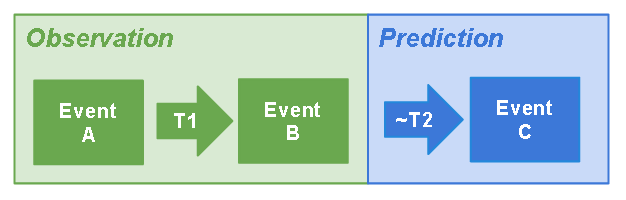
\includegraphics[width=\textwidth]{./img/association_rules.png}
\caption{A general prediction} \label{fig:ass_rule}
\end{figure}


The events forming the \emph{consequent} of our prediction will be alarms raised by the maintenance stations - we want to prevent or be prepared for the alarms happening in the future - and the antecedent can be formed by different kind of elements. Therefore, we will distinguish two main working lines: prediction based on previous alarms (section~\ref{sec:alarm-based-prediction}) and prediction based on external conditions (section~\ref{sec:external}).


\subsection{Prediction based on previous alarms}\label{sec:alarm-based-prediction}
This working line consists of acquiring knowledge on how events are related to each other in terms of occurrence. In other terms, the events in the antecedent of our predictions will be formed by alarms (as well as the consequent, as we said before). Among all the alarms raised on the maintenance stations, some of them may be directly triggered by previous ones, having a direct occurrence relation; or might be caused by the same environmental conditions, being most likely for them to happen along the same time periods. As a result, even in cases where they might seem completely unrelated, the occurrence of one of them can give us information on the chances of others happening within a defined time span.

Our objective is to find and analyse these relations and use them to build useful predictions. Depending on the parameters we use for our knowledge discovery procedures, we might obtain different types of rules. For instance, varying the temporal resolution of our analysis, we might obtain rules to predict events in terms of months, days or hours. Depending on the timespan we work with, our prediction rules may be useful to prevent failures, to be prepared to fix them, or be completely useless if there is not enough anticipation.

It is important to note that in the railway network we are working with, there are different maintenance stations in different railway lines. Neither the maintenance stations or the lines are equal throughout the whole network, and therefore we may have to follow different procedures and expect different results for each of them. Initially, we will treat every station (along with the set of elements under its management) independently, even though we already know their classification and the similarities between them. Unless generalisation is evident and clearly convenient, we will always maintain this separation and obtain a different set of rules for each of them.

Due to the characteristics and large size of the available data, we are likely to find a vast amount of frequent sequences and association rules from which not all of them will be useful for maintenance purposes. Different metrics can be applied to evaluate the \emph{importance} of a rule, such as its confidence (its probability to be true on a given situation), the severity of the predicted events, or its support (absolute frequency of the sequence happening).

A comprehensive analysis is necessary to extract the most useful association rules from the set and discard the others, in order to obtain the most efficient set possible. Additionally, the different metrics can even allow predictions to be filtered in real time, according to the available resources or the desired results.

In figure~\ref{fig:demo_view} we can view an example use case. A maintenance operator could view the alarms which are being raised by the maintenance station (in a similar way as the current systems) and a list of predicted alarms - along with the confidence of the prediction and an estimated time span - based on those past and current alarms.

\begin{figure}[hbtp]
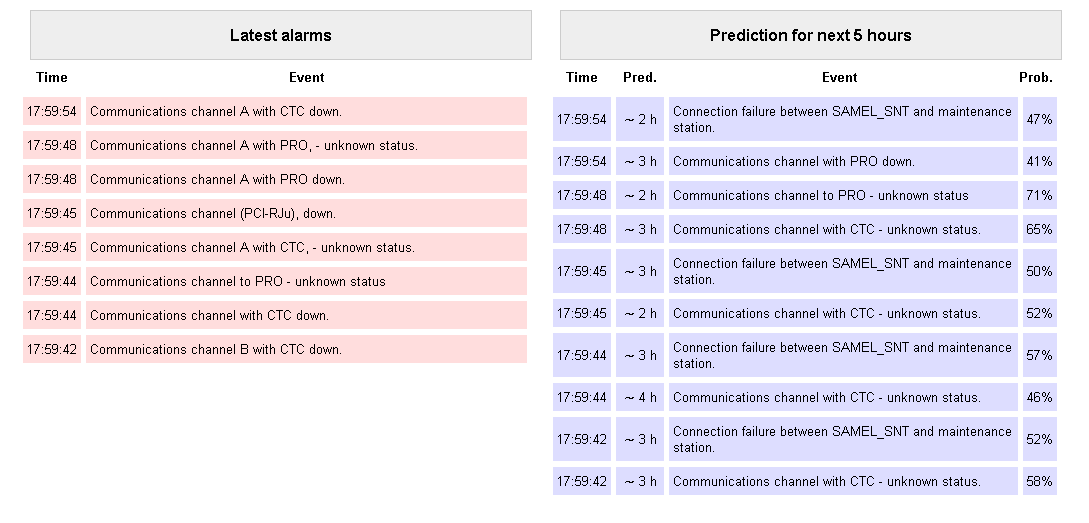
\includegraphics[width=\textwidth]{img/demo_thales.png}
\caption{An example use case} \label{fig:demo_view}
\end{figure}

\subsection{Prediction based on external conditions}\label{sec:external}
This working line consists of acquiring knowledge on the conditions in which alarms are most likely to be raised. The events in the antecedent of our predictions will therefore be variations of different system variables we would have to monitor. This may be the most natural approach for predictive maintenance: trying to observe the environment variations which may be the direct causes of system failures. For example, we might want to analysis which variations of temperature lead to system breakdown, or how slight variations on power supply voltage can indicate a future failure.

However, automatic acquisition of this kind of data is not a trivial issue. With hundreds of elements along the railway lines, and maybe up to dozens of variables to monitor in each of them, it would require an efficient way to obtain this large amount of data.

Currently, the only source of this kind of information we have is the logs maintenance workers fill when performing preventive maintenance procedures. Although we might be able to actually extract useful knowledge from this kind of data, its implementation would not be immediate or easy, as said automatic data acquisition systems would be needed in order for our rules to be applied. For these reasons, we will relegate this kind of predictions to a second place, and focus on alarm-based predictions as mentioned in section~\ref{sec:alarm-based-prediction}.

\section{Knowledge Discovery in Databases}
The whole process we are approaching in this project is usually known as \emph{Data Mining}, or more generally, \emph{Knowledge Discovery in Databases}. A lot of research has been already done on this field which will serve as background for our project, as well as tools and algorithms which have been designed to treat similar problems and which we can adapt or use as base to develop our own.

Knowledge Discovery in Databases - or \emph{KDD} - is a term used to describe the procedure of acquiring high-level knowledge from low-level data. As a formal definition, \emph{Knowledge Discovery} is the non-trivial extraction of implicit, previously unknown, and potentially useful information from data~\cite{Frawley1992}. This knowledge is usually found in the form of patterns and relations between variables which were unlikely to be related.

The KDD process involves several steps~\cite{Feyyad1996} which can be summarized as follows:

\begin{enumerate}
 \litem{Understanding the problem:} The first step involves understanding the environment we are studying and gaining relevant prior knowledge. In this step we must identify which goals we want to set for the knowledge discovery process. This is, we must identify the kind of knowledge we want to obtain and the data we can count on for this process.
 \litem{Creating a target dataset:} We will usually need to select a subset of variables from the available datasets. While the system we are studying may need a lot of variables to log events or make data relations, we will not likely need all of them to characterize our problem. Reducing the dimensionality of the problem will provide better results and ease the following steps.
 \litem{Data cleaning and preprocessing:} In this step we have to discern which data is actually relevant and significant for our study, and which is merely noise or outliers which should be disregarded. Operations such as noise modelling or mapping of missing and unknown values are also taken in this step.
 \litem{Data mining:} For this step we must first have decided the purpose of the model derived by the data mining algorithm. For example, summarization, regression, clustering and others. According to our decision, some data mining algorithms will be more appropriate than others.
 \litem{Interpretation of results:} Consists on interpreting the discovered patterns, removing those redundant or irrelevant and translating the useful ones into understandable terms.
 \litem{Consolidation of discovered knowledge:} The discovered knowledge is finally consolidated in an appropriate form. Depending on the context of our project, it might be simply documented or integrated in predictive modules for the analysed systems.
\end{enumerate}

\emph{Data Mining} comprises a large amount of different algorithms which can be used for the Knowledge Discovery process. Depending on the nature of the data on which we will apply these algorithms, and on the kind of knowledge we expect or want to acquire, we will need algorithms of different types.

Different algorithms can usually be classified in the following categories:

\begin{enumerate}
 \litem{Classification:} Learning a function that maps an item into predefined classes.
 \litem{Regression:} Learning a function that maps an item to a predicted variable.
 \litem{Segmentation:} Identifying a set of clusters to categorise the data.
 \litem{Summarization:} Finding a compact description for the data.
 \litem{Association:} Finding significant dependencies between different variables.\cite{Zhao2003}.
 \litem{Sequence analysis:} Finding frequent sequences or episodes in data~\cite{Zhao2003a,Weiss2002}.
\end{enumerate}

\subsection{Data preprocessing}

Most data mining processes are usually focused on predicting the value of some variables given the value of the rest variables in a given observation. They work with discrete observations for which each of the variables is analysed or predicted. Our case is significantly different, as we have a continuous observation and events which are not modelled as variables. We can easily convert our continuous situation to a discrete one by splitting time into smaller sized periods. Our variables will therefore be the number of times each type of alarm happens during said period, and the time slots will represent the discrete observations. To illustrate this conversion, we have represented an example of the data formats before preprocessing in table~\ref{tab:data_before} and after preprocessing in table~\ref{tab:data_after}.

\begin{table}
\begin{center}
\begin{tabular}{|c|c|c|}
\hline Date & Time & Alarm \\ 
\hline 01-01-2011 & 00:00 & Alarm A \\ 
\hline 01-01-2011 & 00:30 & Alarm B \\ 
\hline 01-01-2011 & 00:45 & Alarm B \\ 
\hline 01-01-2011 & 01:10 & Alarm C \\ 
\hline 01-01-2011 & 01:20 & Alarm A \\ 
\hline 01-01-2011 & 01:30 & Alarm A \\ 
\hline 01-01-2011 & 01:25 & Alarm C \\ 
\hline 01-01-2011 & 02:20 & Alarm A \\ 
\hline 01-01-2011 & 02:30 & Alarm A \\ 
\hline 01-01-2011 & 02:45 & Alarm B \\ 
\hline ... & ... & ... \\ 
\hline 
\end{tabular} 
\end{center} 
\caption {Continuous observation. Example of data in log format.} \label{tab:data_before} 
\end{table}

\begin{table}
\begin{center}
\begin{tabular}{|c|c|c|c|}
\hline Time & Alarm A & Alarm B & Alarm C \\ 
\hline 0 & 1 & 2 & 0 \\ 
\hline 1 & 2 & 0 & 2 \\ 
\hline 2 & 2 & 1 & 0 \\ 
\hline ... & ... & ... & ... \\ 
\hline 
\end{tabular} 
\end{center} 
\caption {Example of discretised data} \label{tab:data_after} 
\end{table}

For further simplification, we can even reduce the problem to terms of whether an alarm happens or not, and disregard the number of times each of them happen. This approach would be necessary when treating alarms which are not very frequent, and for which the number of occurrences during an observation will typically vary between 0 and 1. However, for events with a higher occurrence rate, the actual number of occurrences within an observation might be of importance. The optimum approach might vary between situations, and therefore we cannot still decide for one of them at early stages of the project.

It is also important to note that an optimum choice of the sampling time is important. If we want to achieve predictions in time spans of months, it might be inappropriate to choose an observation period of seconds or minutes. For our project, due to the characteristics of the procedures of railway maintenance, we aim to achieve predictions in terms of weeks. Therefore, we have chosen the observation time to be a period of 24 hours. When working with \emph{sequence analysis}, we have also to define additional time constraints\cite{Suh2011}, such as the maximum distance between the antecedent and consequent, or even between several events on the antecedent (or consequent).

A large amount of existing algorithms have been implemented taking into consideration these issues for sequential analysis~\cite{Wu2010}. Some of them will be analysed in order to work as a base or tool for our project.

\section{Working methods}
For the development of this project, we have found a vast amount of useful tools and software which will provide an inestimable help in the different processes of our work. The main tool used will be the \emph{R} language, a very powerful tool commonly used for handling large amounts of data in an efficient way, and for which a vast amount of tools are available for our needs. R, and the IDE we are using, \emph{RStudio} are open source software and available at no cost.

Due to licensing and compatibility issues, we are not able to use \emph{Microsoft SQL Server} databases to handle data. This is highly inconvenient as the data provided by Thales is in form of MS SQL backup files, which we needed to migrate to a compatible system of our choice: \emph{MySQL}. Given the tabular nature of the data, another solution based on plain text files would not be recommendable - although possible to handle with R - at least at the earliest stages until we analyse all the information and reduce the number of variables to export. In order to perform these migration tasks, a \emph{Windows} platform with \emph{Microsoft SQL Server Express} was required. Migration was successfully possible after slight modification of indexes and field definitions to fix compatibility issues. Once in MySQL format, we can query our data from RStudio without being limited to any kind of platform type or operative system, and will indeed perform further stages of the project under \emph{Unix} platforms.

Among all the available algorithms which can be useful for our project, we have chosen the \emph{cSPADE} algorithm as our starting point. It provides the most straight-away solution for the kind of problem we are approaching, as it considers temporal characteristics and allows us to set time constraints very easily. Other algorithms will be studied and applied at convenience, in order to complement cSPADE and find weak points which we could improve.

Another very useful tools which can be of great help for obtention of this kind of predictions are \emph{Bayesian Networks}\cite{Jensen2009}. A Bayesian network is a probabilistic model which represents a set of variables and their conditional dependencies via a directed acyclic graph. A very simplified example can be seen in figure~\ref{fig:bayesian_example} In our case, it would represent the types of alarms and their relation in a graphical network, allowing us to analyse the probabilities of each of them happening within the current observation. Once an alarm has already been raised, its probability can be set to 100\% in the current observation, allowing us to recalculate probabilities for the rest of alarms by application of Bayes theorem. Bayesian networks can be either directly implemented onto any kind of system - as long as we can have real-time information on risen alarms - or be used to extract rules and implement them onto any other kind of system. There are lots of available tools for working with Bayesian networks. Specifically, we will use \emph{GeNIe/SMILE} as well as \emph{R libraries} for this purpose.

\begin{figure}[hbtp]
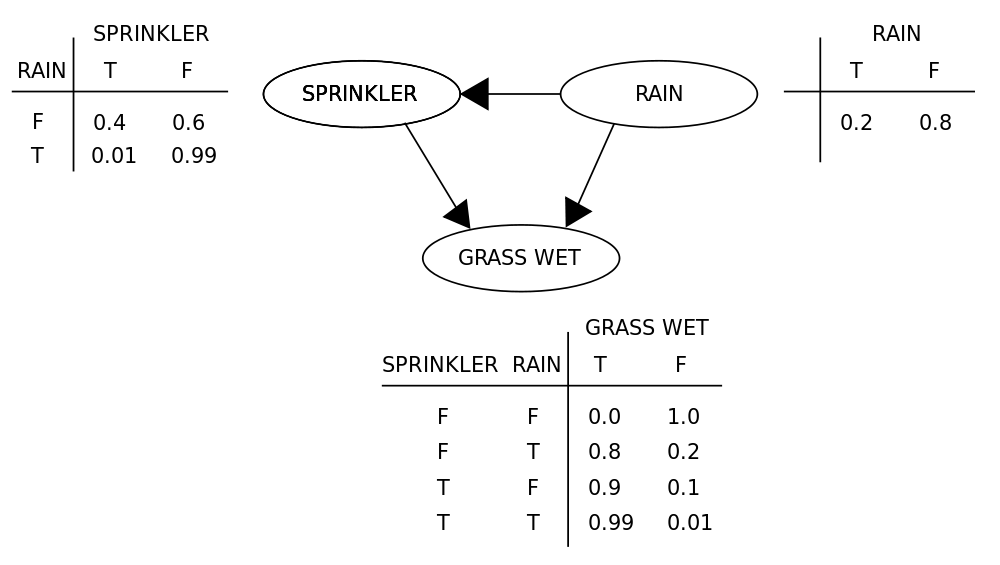
\includegraphics[width=\textwidth]{img/bayesian_example.png}
\caption{An example of a very simple bayesian network} \label{fig:bayesian_example}
\end{figure}


\section{Final comments}
The most important thing before starting any other step, is to completely understand the context and scenario of our project. We do not need to fully know and understand the details on the procedures of railway maintenance, as the nature of the machinery performed reparations is not of significant relevance for the achievement of the defined objectives. In any case where we would need better understanding of system functioning - such as for identifying causal relations between failure events - we would need assistance from expert employees directly related with maintenance.

At this point, we have already treated all received data in order to be able to freely handle it without restrictions from any desired system. Required conversions have been performed and all data is already prepared to be loaded and used in R scripts.

We have also defined the learning objectives for the project, and set a ground to achieve them from an \emph{Knowledge Discovery in Databases} approach. Furthermore, we have made a first insight into \emph{Data Mining} techniques and performed a first analysis on their adequacy for our project. Initial tools have already been selected: cSPADE and GeNIe/SMILE.

In the next stage of Trainmining, we will need to make a deeper insight into the provided databases. The procedures which we have already defined (time discretion and definition of observation times) will have to be performed, selecting the exact variables among all of them which are registered for each alarm.

\clearpage


\bibliographystyle{plain} 
\bibliography{datamining}

\end{document}


